
\section{Datafari}

\subsection{Installation}

Für Datafari musste folgende Software nachinstalliert werden: Java 8 und JQ, ein JSON-Prozessor. Damit die Installation richtig durchläuft, muss die JAVA\_HOME-Variable erstellt werden. Insofern Datafari nicht unter Root laufen soll, muss noch ein besonderer Nutzer mit Root Rechten angelegt werden. Dieser muss wie schon bei Solr höhere User-Limits erhalten. Datafari installiert sich selbst durch eine DEB-Datei. Während der Installation erscheint ein kurzer Setup-Dialog, welcher einen durch die Konfiguration führt. Das Starten des Server geschieht daraufhin durch ein Script im Installationsordner.

\subsection{Indexierung}

Damit eine Indexierung durchgeführt werden kann, muss bei Datafari ein sogenanntes Repository angelegt werden. In diesem wird die Datenbank-Verbindung eingetragen. Dabei ist es wichtig, dass vorher der Treiber korrekt installiert wird. Es kam bei mir dabei zu Problemen. 
Das auf Apache ManifoldCF basierende System akzeptiert nur MySQL-JDBC Treiber. Da der MariaDB-Treiber einen anderen Klassennamen in Java verwendet, funktioniert dieser nicht. \begin{quote} This connection type cannot be configured to work with other databases than the ones listed above without software changes.~\cite[S.~61]{ApacheSoftwareFoundation.}\end{quote} Deswegen musste ich für diesen Test den MySQL-Treiber von Oracle verwendet.
Nachdem der Treiber korrekt installiert ist und das Repository erstellt ist, kann nun einen Job zu Indexierung der Einträge gestartet werden. In diesem werden die Queries und der Zeitplan konfiguriert.
Im ersten Schritt wird das Repository ausgewählt und das Ziel, in diesem Fall also Solr. In dem Tab Queries lassen sich dann diverse Querys bauen. Der erste ist der Seeding Query, welche eine Art Delta-Query für dieses System ist und natürlich der Data-Query, welcher die Daten aus der Datenbank lädt. Dabei werden mehrere Variablen definiert, damit der Query korrekt von ManifoldCF erkannt wird. Zuerst einmal das Feld: IDCOLUMN, welches die ID enthält, dann URLCOLUMN, welches einen Hyperlink für diesen Eintrag enthält. Da hier keine solche Spalte gegeben ist, wird einfach nochmal die ID mitgegeben, was so in einen Screenshot in der Dokumentation zu sehen ist. und als letztes die DATACOLUMN, welche alle Daten konkateniert enthält. Um das System zu testen habe ich allerdings erstmal nur eine Zeile in die DATACOLUMN geschrieben \ref{img:datafariQuery} Die Konkatenation ist vorgegebene die Methode aus der ManifoldCF-Dokumentation. \cite[S.~97]{ApacheSoftwareFoundation.} Dies ist für unseren Zweck leider keine gute Datenstruktur.
Sind alle Querys eingetragen, kann die Indexierung beginnen. Dafür wird der Job in der Oberfläche manuell gestartet, insofern kein Zeitplan konfiguriert ist. In meinen Test kam es dabei allerdings zu Problemen, die Indexierung erfolgte nicht korrekt und blieb immer am Ende hängen. Der Log zeigte ein "Ready for processing" an, machte dort allerdings nicht weiter. Einen Eintrag in der Dokumentation oder generell im Internet konnte ich zu diesem Problem nichts finden. Auch eine Reduktion der Einträge auf nur 125 hat das Problem leider nicht lösen können. Deswegen breche ich an dieser Stelle den Test ab. 

\begin{figure}
	\centering
	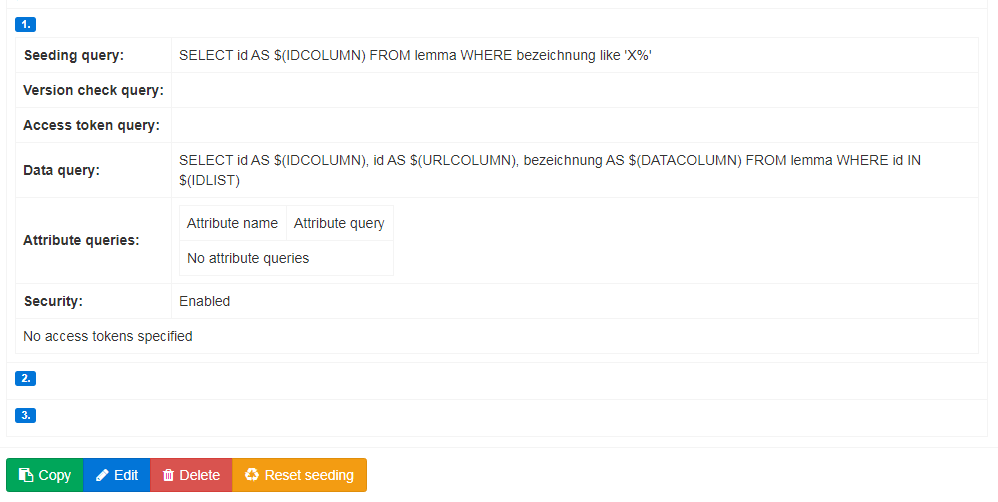
\includegraphics[width=1\linewidth]{images/datafari_query.png}
	\caption{Übersichtsseite des Querys in Datafari.}
	\label{img:datafariQuery}
\end{figure}

\subsection{Oberfläche}

Die Oberfläche von Datafari ist dreigeteilt. Zum einen gibt eine Such-Oberfläche, welche sich ohne Anmeldung erreichen lässt. Als Zweites findet sich eine Administrationsoberfläche, welche erst eingesehen werden kann, sobald man eingeloggt ist. Dort findet man diverse Einstellungen für die Suchmaschinen, wie Synonyme oder die Facetten-Konfiguration. Auch sind dort die Logs einzusehen, welche durch die Einbindung der Oberfläche von Kibana \ref{elasticsearch} aus ELK-Stack angezeigt werden. Die dritte Oberfläche ist die Einstellungsseite für die Datacrawler. Dies ist eine modifizierte Oberfläche von Apache ManifoldCF. Generell sind die Menüs sehr übersichtlich, auch wenn die Einbindung von anderen Anwendungen keine Ideale Lösung darstellt. Es lassen sich keine Updates direkt über die Oberfläche einspielen.
Die Such-Seite und die Seite für die Erstellung der Datacrawler sind Responsive, während die Administrationsoberfläche bei kleineren Bildschirmgrößen das Menü versteckt und die Seite somit unnutzbar macht. Update können auch hier nicht über die Oberfläche eingespielt werden.

\begin{figure}
	\centering
	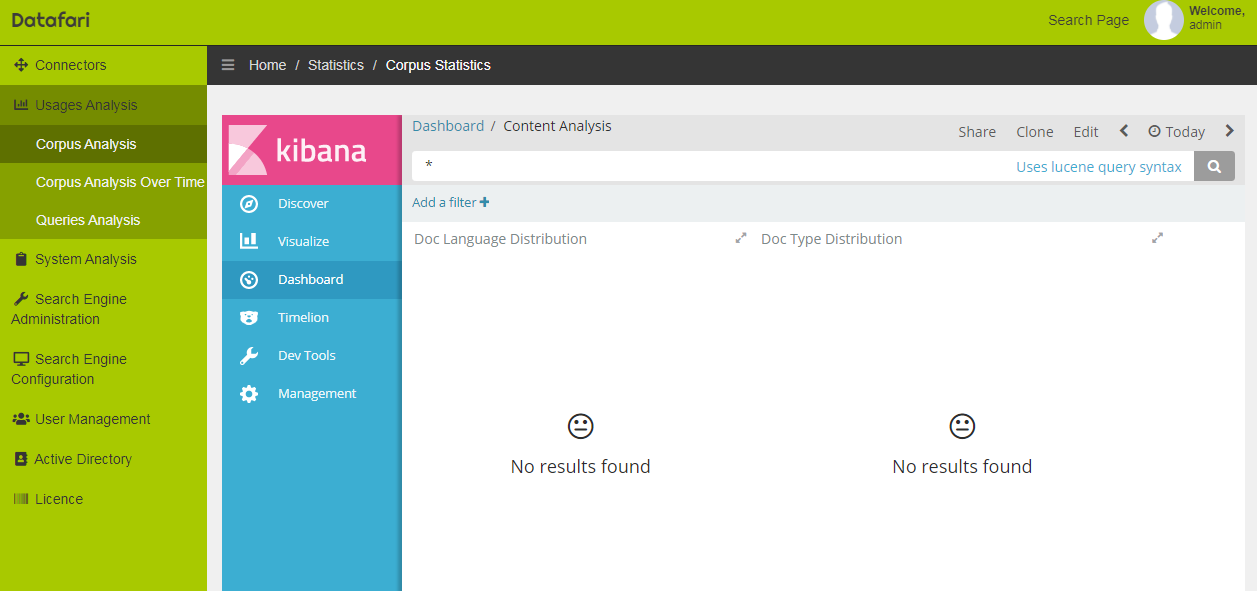
\includegraphics[width=1\linewidth]{images/datafari_kibana.png}
	\caption{Kibana Integration in Datafari.}
	\label{img:datafariKibana}
\end{figure}

\subsection{Dokumentation}

Die Dokumentation geht sehr genau auf die Installation des Systems ein, dabei werden alle Konfigurationsaspekte beleuchtet. Zum Beispiel wird beschrieben, wie die User Limits erhöht werden, oder die JAVA\_HOME-Variable korrekt gesetzt wird. Allerdings merkt man an manchen Stellen, dass die Dokumentation nicht von nativen Englischsprechenden geschrieben wurde, da die Grammatik nicht immer stimmt. Allerdings hat dies nie zu Problemen oder Verwechslungen geführt.
Bei der Dokumentation zum Einrichten des JDBC-Treibers finden sich einige Probleme \ref{img:datafariJDBC}. Zum einen sind beide Pfade, die in dem Text angegeben sind, falsch. Einer davon wird sogar richtig in dem Screenshot direkt darunter angezeigt. Und zum anderen ist der zweite Screenshot so niedrig aufgelöst, dass sich nicht viel erkennen lässt. Dies passiert auch, wenn das Bild in einen neuen Tab geladen wird. Generell ist die Dokumentation für den Umgang mit Datenbanken nicht sehr ausführlich. Die Erklärungen, wofür die Variables bei der Erstellung eines Jobs stehen, musste ich in der Dokumentation von ManifoldCF nachlesen.
Die Dokumentation ist im aktuellen Stand nicht sauber strukturiert. Sie gibt das Gefühl, dass es sich eher um eine Sammlung verschiedener Artikel, welche Intern genutzt wurden, handelt.

\begin{figure}
	\centering
	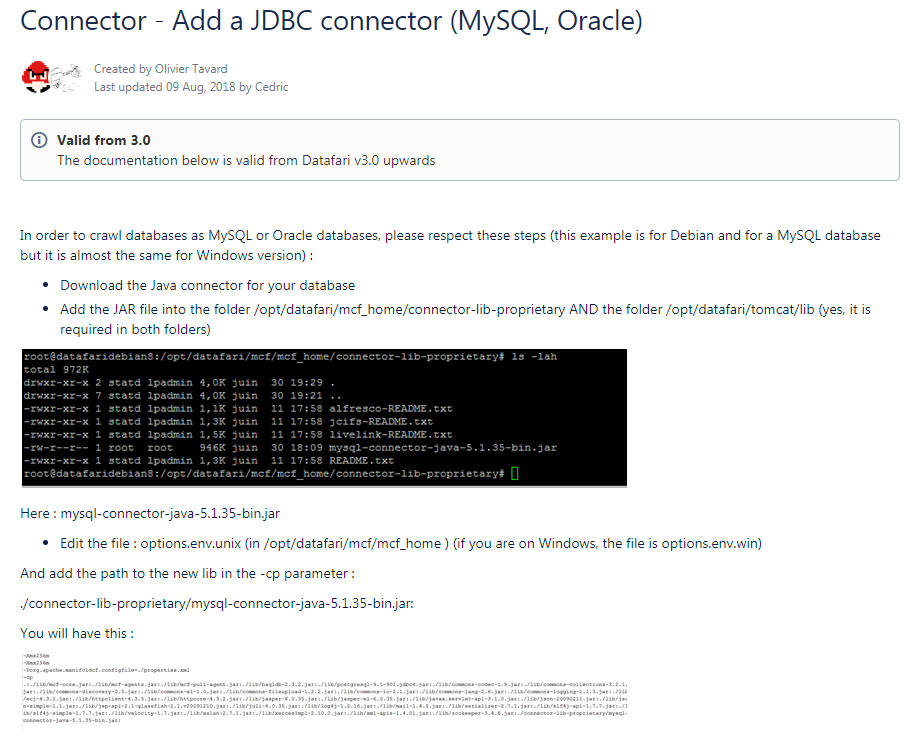
\includegraphics[width=1\linewidth]{images/datafari_doku_wrong_path.png}
	\caption{Dokumentationsseite für den JDBC Treibers von Datafari.}
	\label{img:datafariJDBC}
\end{figure}


\subsection{Absetzen einer Anfrage und Integration in PHP}

Durch das fehlgeschlagene Einlesen der Daten konnte dieser Test leider nicht ausgeführt werden.
